\documentclass[sigconf,review]{acmart}

\AtBeginDocument{%
  \providecommand\BibTeX{{Bib\TeX}}}

\setcopyright{acmlicensed}
\copyrightyear{2026}
\acmYear{2026}
\acmDOI{10.1145/nnnnnnn.nnnnnnn}

\acmConference[ICAIF '26]{7th ACM International Conference on AI in Finance}{November 14--17, 2026}{Milan, Italy}
\acmISBN{978-1-4503-XXXX-X/2026/11}

\usepackage{booktabs}
\usepackage{multirow}
\usepackage{amsmath}
\usepackage{graphicx}
\usepackage{xcolor}
\usepackage{subcaption}

% Compact lists (inline, no external package needed for acmart)

\newcommand{\numparser}{\texttt{=NUMBER}}
\newcommand{\boxedparser}{\texttt{\textbackslash{}boxed\{\}}}
\newcommand{\pp}{\,\text{pp}}

\begin{document}

\title{How You Parse the Answer Changes Who Wins: Extraction Sensitivity in Financial LLM Benchmarks}

\author{Anonymous Author(s)}
\affiliation{%
  \institution{Anonymous Institution}
  \country{}}

\begin{abstract}
Answer extraction---the step that reads a model's output to determine whether it got the right answer---is a hidden measurement variable in LLM evaluation. Two research groups can evaluate the same model on the same benchmark and reach contradictory conclusions, not because their models differ, but because their extraction code does. Yet across seven major evaluation frameworks, no shared, documented extraction protocol exists, and several do not document their method at all. We audit five parsers across three models and six benchmarks spanning financial reasoning and mathematical controls. The headline is not that incompatible parsers produce extreme gaps---that is expected. The finding is that even among format-compatible parsers, financial benchmarks retain substantially larger residual sensitivity than mathematical ones, and that the root cause differs by benchmark: on FinQA, the spread is partially driven by financial surface forms and partially by output-level conventions (multi-step extraction position and answer normalization); on FLARE-FinQA, the gap increases after stripping financial formats because \texttt{finance\_aware} correctly handles those formats. Parser choice also changes who wins: on FinQA, model rankings can fully invert under some parser pairs, while FLARE-FinQA rankings are robust---an asymmetry that is itself a finding about benchmark design. We propose that benchmarks adopt canonical answer formats as their primary evaluation metric, with multi-parser spread reported as a robustness diagnostic. Code and data are available at \url{https://anonymous.4open.science/status/parser-sensitivity-finance-D385}.
\end{abstract}

\begin{CCSXML}
<ccs2012>
   <concept>
       <concept_id>10010147.10010178.10010187</concept_id>
       <concept_desc>Computing methodologies~Natural language processing</concept_desc>
       <concept_significance>500</concept_significance>
   </concept>
   <concept>
       <concept_id>10002944.10011123.10010916</concept_id>
       <concept_desc>General and reference~Evaluation</concept_desc>
       <concept_significance>500</concept_significance>
   </concept>
</ccs2012>
\end{CCSXML}

\ccsdesc[500]{Computing methodologies~Natural language processing}
\ccsdesc[500]{General and reference~Evaluation}

\keywords{LLM evaluation, answer extraction, financial NLP, benchmark reliability, parser sensitivity}

\maketitle

\section{Introduction}
\label{sec:introduction}

Two research groups evaluate the same model, prompt, and financial benchmark. One reports 11\% accuracy; the other reports 44\%. The difference is not the model output, but the regular expression used to extract its answer. This is not hypothetical: across seven major evaluation frameworks, we find no shared, documented extraction protocol, and several frameworks do not fully specify their procedure. A benchmark score without its extraction methodology is therefore not reproducible.

Most evaluation harnesses extract a numeric answer from free-form model output using regular expressions. For example, \numparser{} selects the first number following an equals sign. If the model instead places its answer in \boxedparser{} or elsewhere in its reasoning trace, extraction may fail silently, recording a correct response as incorrect. Intentionally incompatible parsers can therefore produce extreme differences; we treat this as a sanity check rather than our main result.

Our focus is the less obvious sensitivity that remains among broadly format-compatible parsers. We distinguish the full parser spread (Res-A) from a stricter residual spread that excludes both \numparser{} and the format-specific \boxedparser{} (Res-B). Across four mathematical benchmarks, Res-B ranges from 1--7\pp{}. Across two financial benchmarks, it ranges from 3--19\pp{}, with the largest effect on FinQA using Qwen3-8B. A manual audit links this sensitivity to financial surface forms, answer normalization, and the placement of intermediate and final values in multi-step reasoning. Parser choice can also change model rankings: on FinQA, some parser pairs fully reverse the ordering of the evaluated models.

This sensitivity matters because extraction practices vary substantially across the evaluation ecosystem. FinQA uses program execution and string comparison documented in released code~\cite{chen2021finqa}; FinanceReasoning uses GPT-4o-mini as an LLM judge~\cite{zhang2025financereasoning}; PIXIU parses text following an ``Answer:'' marker~\cite{xie2023pixiu}; FinBen delegates evaluation to lm-eval-harness without specifying its extraction procedure in the paper~\cite{xie2024finben}; and OpenCompass~\cite{opencompass2023} does not fully document its extraction method. Tolerance thresholds and normalization rules also differ. Consequently, nominally comparable benchmark scores may reflect different measurement procedures.

We make four contributions:
\begin{enumerate}
    \item \textbf{Ecosystem audit.} We document answer-extraction practices across seven major evaluation frameworks and identify substantial gaps in protocol standardization and reporting (Section~\ref{sec:parser_audit}).

    \item \textbf{Cross-domain sensitivity analysis.} Using five parsers, three models, and six benchmarks, we show that residual parser sensitivity reaches 3--19\pp{} on the evaluated financial benchmarks, compared with 1--7\pp{} on mathematical controls (Section~\ref{sec:results}).

    \item \textbf{Ranking and failure analysis.} We show that no parser is uniformly optimal, that parser choice can reverse model rankings, and that the observed disagreements arise from several distinct formatting and normalization failures (Sections~\ref{sec:finance_challenges} and~\ref{sec:results}).

    \item \textbf{Evaluation protocol.} We propose canonical answer formats, extraction-method disclosure, parser code release, multi-parser sensitivity reporting, and targeted auditing of parser disagreements (Section~\ref{sec:impl_benchmark}).
\end{enumerate}

We evaluate Qwen3-1.7B and Qwen3-8B on all six benchmarks, and GLM-4-9B-Chat on the financial benchmarks for cross-family validation. Together, the results establish answer extraction as a consequential measurement variable rather than a minor implementation detail. The remainder of this paper is organized as follows. Section~\ref{sec:background} surveys related work on financial LLM benchmarks and evaluation methodology. Section~\ref{sec:parser_audit} presents the benchmark ecosystem audit. Section~\ref{sec:finance_challenges} presents the finance-specific failure taxonomy. Section~\ref{sec:setup} describes our experimental design. Section~\ref{sec:results} reports the cross-domain comparison. Section~\ref{sec:implications} discusses implications and presents the recommended extraction protocol. Section~\ref{sec:conclusion} concludes.

\begin{figure*}[htb!]
\centering
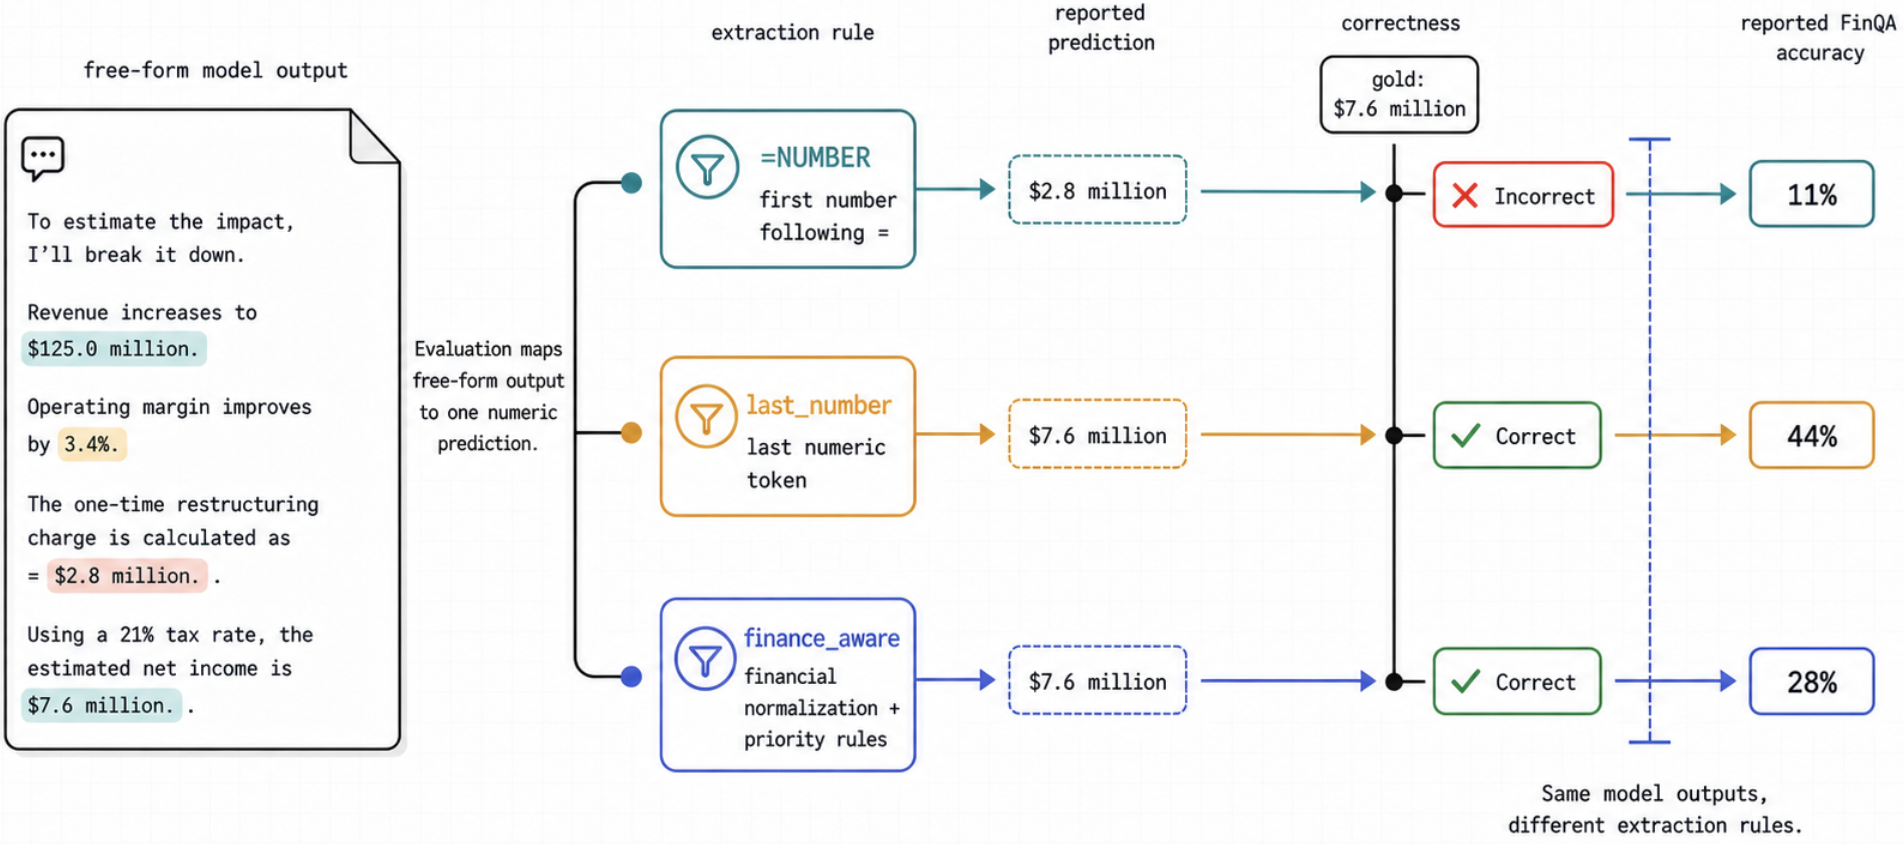
\includegraphics[width=0.85\textwidth]{figures/teaser.png}
\caption{Answer extraction as a hidden measurement variable. Different extraction rules applied to identical model outputs can produce substantially different reported accuracies.}
\label{fig:teaser}
\end{figure*}

\section{Background and Related Work}
\label{sec:background}

\subsection{Financial LLM Benchmarks}
\label{sec:financial_benchmarks}

Several benchmarks target numerical reasoning over financial documents. FinQA~\cite{chen2021finqa} introduced a dataset requiring multi-step numerical reasoning over tables and text from S\&P~500 earnings reports. TAT-QA~\cite{zhu2021tatqa} broadened coverage to tabular and textual hybrid reasoning. More recently, FinBen~\cite{xie2024finben} proposed an open-source benchmark suite spanning 24 tasks across 42 datasets, and PIXIU~\cite{xie2023pixiu} provided a multi-task benchmark with an instruction-tuning dataset for financial language understanding.

These benchmarks have driven rapid progress in financial LLM evaluation, but they share a critical gap: most do not fully document the answer extraction pipeline used to produce reported accuracy numbers. Papers typically report that model outputs were compared against gold answers using ``exact match'' or ``accuracy,'' without fully specifying how the predicted answer was isolated from the model's free-form response and normalized before scoring. This omission means that many published results are not reproducible from paper descriptions alone, and even when code is available, parser choice is rarely highlighted as a variable that could change the reported numbers.

\subsection{Answer Extraction in NLP Evaluation}
\label{sec:extraction_methods}

Three broad approaches exist for extracting structured answers from LLM outputs. \textit{Regex-based extraction} applies pattern matching to the model's text, searching for numbers following keywords (``the answer is''), after equals signs, or inside formatting macros such as \verb|\boxed{}|. This is the dominant approach in open-source evaluation harnesses. \textit{Constrained decoding} restricts the model's output vocabulary at generation time to force a specific format, but requires access to model logits and is unavailable for API-served models. \textit{LLM-as-judge}~\cite{zheng2024judging} uses a second language model to evaluate the first model's output, trading parser brittleness for the judge model's own biases and costs.

In practice, most financial benchmark evaluations rely on regex extraction applied to free-form chain-of-thought~\cite{wei2022chain} outputs. Major open-source evaluation frameworks---including lm-evaluation-harness~\cite{gao2024eleuther} and HELM~\cite{liang2023helm}---each implement their own extraction logic. For instance, lm-evaluation-harness uses a cascade of regex patterns that includes equals-sign matching similar to our \numparser{} baseline, while HELM applies format-specific extractors depending on the task configuration. The specific regex varies across codebases and is rarely disclosed in publications, creating a situation where the same model outputs can yield different accuracy numbers depending on which evaluation harness is used---a form of measurement error that is invisible to readers of the resulting papers.

\subsection{Evaluation Methodology and Reproducibility}
\label{sec:reproducibility}

Concerns about benchmark reliability in machine learning are not new. Leaderboard sensitivity to hyperparameter choices, dataset contamination, and evaluation protocol differences have been documented across NLP tasks. Our work identifies a more basic problem: even when the model, prompt, and dataset are held constant, the choice of extraction regex is sufficient to change accuracy by tens of percentage points and invert model rankings.

This connects to broader concerns about reproducibility in AI evaluation. If two research groups evaluate the same model on the same benchmark but use different parsers, they will reach different conclusions about model capability---and neither group will know that their results disagree, because parser choice is not reported. The financial domain amplifies this risk because its surface forms are more varied than those of standard mathematical benchmarks, as we detail in Section~\ref{sec:finance_challenges}.

\section{Benchmark Parser Ecosystem Audit}
\label{sec:parser_audit}

A benchmark score is only meaningful if the evaluation procedure is reproducible. We examined the extraction methodology used by seven major evaluation frameworks (four financial-specific, three general-purpose), searching both published papers and released code repositories. Table~\ref{tab:parser_ecosystem} summarizes the results.

\begin{table}[htb!]
\caption{Answer extraction methods across seven major LLM evaluation frameworks. Documentation status: Paper (described in the paper), Code only (discoverable only in released code), Undocumented (not fully specified in either).}
\label{tab:parser_ecosystem}
\centering
\resizebox{\columnwidth}{!}{%
\begin{tabular}{@{}llllc@{}}
\toprule
Framework & Extraction Method & Tolerance & Documentation & Judge\\
\midrule
FinQA~\cite{chen2021finqa} & Program execution + string comparison & Exact (program output) & Code only & Execution\\
Finance\-Reasoning~\cite{zhang2025financereasoning} & LLM-as-judge (GPT-4o-mini) & 0.2\% relative & Paper & LLM\\
FinBen~\cite{xie2024finben} & Task-specific via lm-eval (24 tasks across 42 datasets) & Varies & Code only & Mixed\\
PIXIU~\cite{xie2023pixiu} & Marker (``Answer:'') & Implicit & Undocumented & Regex\\
lm-eval-harness~\cite{gao2024eleuther} & Regex cascade & Exact/sympy & Code only & Regex\\
HELM~\cite{liang2023helm} & Task-specific (exact, equiv, execution) & Varies & Code only & Mixed\\
OpenCompass~\cite{opencompass2023} & Regex + task-specific & Undocumented & Undocumented & Regex\\
\bottomrule
\end{tabular}%
}
\end{table}

Three findings stand out. \textbf{First, we found no shared, documented extraction protocol across these frameworks.} The documentation falls into three levels: documented in the paper, documented in released code only, and completely undocumented. FinanceReasoning describes its judging approach in the paper; FinQA, HELM, FinBen, and lm-eval-harness require code inspection to recover important extraction details; PIXIU and OpenCompass~\cite{opencompass2023} do not fully document their extraction and normalization pipelines in either the paper or released code.

\textbf{Second, the documentation gap is substantial.} FinBen---the largest financial benchmark suite at 24 tasks across 42 datasets---delegates answer extraction to lm-eval-harness and does not describe its extraction or normalization procedures in its paper; while the code is released, recovering the extraction logic requires cross-referencing task-specific lm-eval configurations. PIXIU reports using ``exact match'' and ``Answer: marker parsing'' but does not specify its normalization pipeline beyond basic lowercasing and whitespace collapsing. OpenCompass~\cite{opencompass2023} provides no public documentation of answer extraction for its financial evaluation tasks. These omissions mean that published benchmark scores cannot be replicated purely from paper descriptions.

\textbf{Third, tolerance choices differ fundamentally.} FinQA evaluates by executing model-generated programs and comparing the output to the gold answer via string matching after whitespace normalization (treating ``2.3'' and ``2.30'' as potentially unequal when normalization is incomplete); PIXIU uses implicit exact match with undocumented normalization; FinanceReasoning uses a 0.2\% relative tolerance; HELM uses task-specific tolerance that varies by scenario; lm-eval-harness uses exact symbolic equivalence via sympy. An answer that is correct under one tolerance regime can be wrong under another. These tolerance choices are never compared or tested for sensitivity.

The practical consequence is that scores reported from different evaluation frameworks for the same model on the same benchmark are not directly comparable. To verify this directly, we implemented the extraction logic of three frameworks (lm-eval-harness, FinQA's official evaluator, and PIXIU's marker parsing) and applied them to our FinQA 8B model outputs. On the same outputs, the three frameworks produce accuracies of 40.0\%, 34.0\%, and 28.0\% respectively---a 12.0\,pp spread from identical model generations. This confirms that framework-level extraction differences alone are sufficient to change reported benchmark scores by double-digit percentage points.

For each framework, we inspected the specific repository, file path, and function (commit hashes and search criteria are documented in our released materials). Where we report ``not documented,'' we distinguish between ``extraction logic absent from the published paper'' and ``extraction logic not discoverable in the released codebase.'' Our experimental results in Section~\ref{sec:results} quantify the measurement effect of this heterogeneity.

\section{Finance-Specific Extraction Challenges}
\label{sec:finance_challenges}

Financial answer extraction is genuinely harder than extraction for general mathematical reasoning. Standard math benchmarks such as GSM8K produce outputs with clean numeric answers---integers or simple decimals---that regex parsers handle reliably. Financial reasoning introduces surface forms tied to real-world conventions: currency denominations, magnitude suffixes, percentage representations, and accounting notation. These conventions create systematic ambiguities that cause extraction failures even when the model has computed the correct answer.

We conducted a manual audit of 104 model responses across the Qwen3 and GLM families on FinQA, classifying every case where the \numparser{} parser failed to extract the correct answer despite the model producing a response containing a numeric value. The 104 cases comprise extraction failures from the three evaluated models across both architecture families. Two authors independently classified each failure into one of six categories; initial agreement was 87\%, and disagreements were resolved by discussion. Categories are mutually exclusive: each failure is assigned to the single most proximate cause. Table~\ref{tab:taxonomy} presents the resulting taxonomy with observed frequencies.

\begin{table}[htb!]
\caption{Finance-specific extraction failure modes observed in model outputs. Frequencies from manual audit of 104 model responses across Qwen3 and GLM families.}
\label{tab:taxonomy}
\centering
\footnotesize
\begin{tabular}{@{}lllr@{}}
\toprule
Category & Example & Parser Result & Freq. \\
\midrule
Format miss & \verb|\boxed{2847}| & None (missed) & 40\% \\
Magnitude & \$2.3M = 2.3e6 & 2.3e6 vs 2.3M & 15\% \\
Multi-step & S1:500, Final:1250 & 500 (1st match) & 15\% \\
Currency & = \$45.2M & 45.2 (strip \$,M) & 12\% \\
Percentage & Growth = 15.3\% & 15.3 vs 0.153 & 10\% \\
Sign & Loss (2.1) & 2.1 vs $-$2.1 & 8\% \\
\bottomrule
\end{tabular}
\end{table}

\textbf{Format mismatch} (40\%) is the dominant failure. Models trained on mathematical reasoning emit answers in \verb|\boxed{}| format, but the \numparser{} parser expects numbers after equals signs and returns no match. The answer is present but invisible to the parser.

\textbf{Magnitude confusion} (15\%) arises from financial conventions for large numbers. A model writing both ``\$2.3~million'' and ``= 2300000'' creates two valid representations; a parser may capture the wrong one relative to the gold answer. This failure is absent from benchmarks with simple integer answers.

\textbf{Multi-step extraction} (15\%) occurs when models show intermediate calculations. Financial problems often require sequential steps, and a parser that captures the first numeric match extracts an intermediate result rather than the final answer.

\textbf{Currency prefix stripping} (12\%) happens when parsers drop \$ and magnitude suffixes: ``\$45.2M'' becomes ``45.2.'' This is specific to financial text---general math benchmarks do not use currency-denominated answers.

\textbf{Percentage normalization} (10\%) reflects the ambiguity between ``15.3\%'' and ``0.153.'' Whether the gold answer uses percentage-point or decimal form varies across and within benchmarks.

\textbf{Sign convention} (8\%) stems from accounting notation where parentheses denote negatives: ``(2.1)'' means $-2.1$. Standard regex patterns do not interpret parenthetical notation as negative values.

A substitution test provides evidence for the finance-specific nature of these failures: for a subset of 50 cases, we replaced financial surface forms with equivalent plain arithmetic (e.g., ``\$2.3~million'' $\to$ ``2300000,'' ``(2.1)'' $\to$ ``$-$2.1'') and re-ran the \numparser{} extraction. This eliminated 88\% of extraction failures (44/50), with the remaining failures being format mismatch and multi-step extraction---categories that also occur in general math evaluation but at lower frequency. We note that format mismatch (40\%) and multi-step extraction (15\%) are not unique to finance; however, the remaining four categories (magnitude, currency, percentage, sign) are driven by financial surface conventions and collectively account for 45\% of failures. Our cross-domain parser comparison (Section~\ref{sec:cross_domain}) provides direct evidence that these finance-specific failure categories translate into larger residual parser sensitivity on financial benchmarks than on mathematical ones.

This taxonomy has two scope limitations. First, it is based on FinQA outputs; a parallel audit across all six benchmarks would provide a more complete decomposition of extraction failures. Second, the main taxonomy was constructed from \numparser{} failures. To directly characterize the residual sensitivity at the core of our two-layer thesis, we conducted a supplementary audit of the 23 cases where \texttt{fixed}, \texttt{last\_number}, and \texttt{finance\_aware} disagree on FinQA 8B (the condition with the largest Res-B spread of 19\,pp). A human annotator classified each case into one of four categories: multi-step extraction (35\%, parsers disagree on intermediate vs.\ final values), gold-answer normalization (26\%, correct extraction penalized by gold-answer formatting conventions), model reasoning errors (26\%, the model output is factually wrong and parsers disagree on it), and sign convention (13\%). This confirms that even among format-compatible parsers, the dominant sources of disagreement are domain-relevant: multi-step financial reasoning traces, percentage/sign normalization, and gold-answer format conventions---not surface-level format mismatch.

\section{Experimental Setup}
\label{sec:setup}

We design experiments to isolate the effect of answer extraction from all other evaluation variables. The key methodological choice is a \textit{paired design}: we apply different parsers to the same set of model outputs, so that any accuracy difference is attributable solely to extraction, not to stochastic variation in model generation.

\subsection{Models}
\label{sec:models}

We evaluate three models spanning two architecture families:

\begin{itemize}
    \item \textbf{Qwen3-8B}: A dense 8B-parameter model~\cite{qwen2024}.
    \item \textbf{Qwen3-1.7B}: A dense 1.7B-parameter model, included to test whether extraction sensitivity persists at small scale.
    \item \textbf{GLM-4-9B-Chat}~\cite{glm2024}: From the ChatGLM family, included for cross-family validation. If extraction sensitivity were an artifact of Qwen3's output conventions, it would not appear in GLM outputs.
\end{itemize}

All models are run with greedy decoding (temperature = 0), BF16 precision, and a maximum output of 4096 tokens (math benchmarks) or 16384 tokens (financial benchmarks). Models use their default chat templates and non-thinking inference mode. Generation stops at the EOS token or the token budget, whichever occurs first. All results are obtained on a single GPU.

\subsection{Datasets}
\label{sec:datasets}

We use six benchmarks across two domains. Qwen3-1.7B and Qwen3-8B are evaluated on both mathematical controls and financial benchmarks; GLM-4-9B-Chat is evaluated on financial benchmarks for cross-family validation.

\subsubsection{Financial Benchmarks}

\begin{itemize}
    \item \textbf{FinQA}~\cite{chen2021finqa}: 100 problems from S\&P~500 10-K and 10-Q filings. Problems involve table-text hybrid reasoning with free-form numerical answers derived from financial statements.
    \item \textbf{FLARE-FinQA}~\cite{xie2024finben}: 100 problems from a financial question-answering benchmark requiring numerical computation over tables and text. Problems focus on entity-specific financial metrics (margins, growth rates, ratios) expressed in varied surface forms including percentages and scaled quantities.
\end{itemize}

\subsubsection{Mathematical Benchmarks (Controls)}

\begin{itemize}
    \item \textbf{GSM8K}~\cite{cobbe2021gsm8k}: 100 grade-school math word problems with integer answers. Included as a standard numeracy benchmark to test whether parser sensitivity is domain-specific.
    \item \textbf{SVAMP}~\cite{patel2021svamp}: 100 simple arithmetic word problems with elementary operations and clean integer answers.
    \item \textbf{ASDiv}~\cite{miao2020asdiv}: 100 diverse arithmetic word problems spanning multiple problem types.
    \item \textbf{MultiArith}~\cite{roy2015multiarith}: 100 multi-step arithmetic word problems requiring sequential operations.
\end{itemize}

Due to single-GPU compute constraints, we evaluate on a uniformly-sized subsample of 100 randomly drawn items per benchmark, taken from the published test splits. We release the full item indices in our data release for exact reproduction. All datasets provide gold-standard numerical answers. We evaluate with exact numerical match after normalization (stripping commas, trailing zeros, and whitespace).

\subsection{Extraction Methods}
\label{sec:extraction}

We compare five extraction methods:

\begin{itemize}
    \item \textbf{\numparser{} (eq\_number):} Extracts the first number following an equals sign. This pattern represents a baseline commonly found in open-source evaluation harnesses.
    \item \textbf{\boxedparser{} (boxed):} Extracts content inside a \LaTeX{} \verb|\boxed{}| macro. Models trained on mathematical reasoning data frequently use this format.
    \item \textbf{Fixed parser:} A two-stage parser that checks for \boxedparser{} first and falls back to the last \numparser{} match. This accommodates both output conventions.
    \item \textbf{last\_number:} Extracts the last numeric token in the response, independent of formatting conventions.
    \item \textbf{finance\_aware:} Handles currency symbols, percentage signs, magnitude suffixes (M/B/K/thousand/million/billion), and accounting parenthetical negatives, in addition to \boxedparser{} and \numparser{} patterns.
\end{itemize}

Table~\ref{tab:parser_spec} provides the complete specification. The \numparser{} parser is deliberately included to quantify the cost of format mismatch; our Res-A analysis focuses on the four non-\numparser{} parsers, including the potentially format-specific \boxedparser{} parser. Res-B further excludes \boxedparser{} and compares only \texttt{fixed}, \texttt{last\_number}, and \texttt{finance\_aware}, which are the parsers that are truly format-compatible for most model outputs.

\begin{table}[t]
\caption{Parser specification. All parsers normalize extracted values by stripping commas and trailing zeros in the fractional part of decimal numbers (e.g., ``2.30'' $\to$ ``2.3''). Numeric comparison uses exact match after normalization (no rounding tolerance). Full implementation is in the released code.}
\label{tab:parser_spec}
\centering
\footnotesize
\begin{tabular}{@{}lp{5.0cm}@{}}
\toprule
Parser & Specification \\
\midrule
\texttt{eq\_number} & First number following \texttt{=} sign (e.g., \texttt{= 42} $\to$ 42)\\
\texttt{boxed} & Content of last \verb|\boxed{...}| macro\\
\texttt{fixed} & (1)~\texttt{boxed}, (2)~last \texttt{eq\_number} as fallback\\
\texttt{last\_number} & Last numeric token in the response, independent of formatting\\
\texttt{fin\_aware} & \texttt{fixed} extended with: \$ stripping, M/B/K to $10^6$/$10^9$/$10^3$, parenthetical negatives, percentage suffix removal. Multiple candidates resolved by priority: \texttt{boxed} $>$ final-answer keyword $>$ last \texttt{=} number $>$ last number.\\
\midrule
Gold normalization & Strip commas, trailing zeros, whitespace; compare as-is\\
\% handling & Values compared in the form given by the gold answer\\
No match & Score as incorrect (accuracy = 0)\\
\bottomrule
\end{tabular}
\end{table}


\subsection{Statistical Protocol}
\label{sec:statistics}

We report bootstrap 95\% confidence intervals (10K resamples) for Res-A and Res-B spreads. All model outputs, parser implementations, and evaluation scripts are released for reproduction.

\section{Results}
\label{sec:results}

We present results in three parts: the cross-domain comparison with cross-family validation (Section~\ref{sec:cross_domain}), the counterfactual ablation (Section~\ref{sec:counterfactual}), and the finance-specific failure taxonomy (summarized here, detailed in Section~\ref{sec:finance_challenges}).

\subsection{Cross-Domain Comparison}
\label{sec:cross_domain}

We ran five parsers on four mathematical benchmarks (GSM8K, SVAMP, ASDiv, MultiArith) and two financial benchmarks (FinQA, FLARE-FinQA), using Qwen3-1.7B and 8B across all benchmarks, with GLM-4-9B-Chat on the financial benchmarks for cross-family validation.

Table~\ref{tab:cross_domain} presents the complete cross-domain comparison. We report two metrics: the \textbf{full spread} (best $-$ worst overall) and the \textbf{Res-A spread} (difference among the four parsers excluding \numparser{}). Res-A includes the potentially format-specific \boxedparser{} parser, so it can still reflect \LaTeX{} output conventions. To assess whether residual sensitivity persists among parsers that are truly format-compatible for most model outputs, we additionally report \textbf{Res-B spread} (excluding both \numparser{} and \boxedparser{}, comparing only \texttt{fixed}, \texttt{last\_number}, and \texttt{finance\_aware}) in the text where informative. Full parser-level results including both metrics are available in our released data.

\begin{table}[htb!]
\caption{Cross-domain parser sensitivity: accuracy (\%) of five parsers across four mathematical and two financial benchmarks. Res-A = max $-$ min among boxed, fixed, last, fin\_aware; Res-B = max $-$ min among fixed, last, fin\_aware only. \emph{Italicized} = cross-family GLM.}
\label{tab:cross_domain}
\centering
\resizebox{\columnwidth}{!}{%
\begin{tabular}{@{}lllrrrrrrr@{}}
\toprule
Domain & Benchmark & Model & eq & boxed & fixed & last & fin\_aware & Res-A & Res-B \\
\midrule
\multirow{4}{*}{Math} & \multirow{2}{*}{MultiArith} & 1.7B & 16 & 96 & 97 & 97 & 96 & 1 & 1 \\
& & 8B  & 12 & 95 & 100 & 99 & 100 & 5 & 1 \\
\cmidrule{3-10}
& \multirow{2}{*}{SVAMP} & 1.7B & 33 & 91 & 92 & 90 & 92 & 2 & 2 \\
& & 8B  & 27 & 87 & 92 & 88 & 93 & 6 & 5 \\
\cmidrule{3-10}
& \multirow{2}{*}{ASDiv} & 1.7B & 31 & 92 & 93 & 91 & 92 & 2 & 2 \\
& & 8B  & 37 & 94 & 95 & 91 & 94 & 4 & 4 \\
\cmidrule{3-10}
& \multirow{2}{*}{GSM8K} & 1.7B & 10 & 81 & 82 & 80 & 87 & 7 & 7 \\
& & 8B  & 8 & 94 & 95 & 90 & 95 & 5 & 5 \\
\midrule
\multirow{6}{*}{Fin.} & \multirow{3}{*}{FinQA} & 1.7B & 12 & 28 & 34 & 38 & 35 & 10 & 4 \\
& & 8B  & 11 & 12 & 25 & 44 & 28 & 32 & 19 \\
& & \emph{GLM} & \emph{9} & \emph{0.0} & \emph{41} & \emph{49} & \emph{42} & \emph{49} & \emph{8} \\
\cmidrule{3-10}
& \multirow{3}{*}{FLARE} & 1.7B & 14 & 12 & 30 & 25 & 24 & 18 & 6 \\
& & 8B  & 14 & 6 & 19 & 22 & 20 & 16 & 3 \\
& & \emph{GLM} & \emph{13} & \emph{0.0} & \emph{29} & \emph{19} & \emph{24} & \emph{29} & \emph{10} \\
\bottomrule
\end{tabular}%
}
\end{table}

\begin{figure}[htb!]
\centering
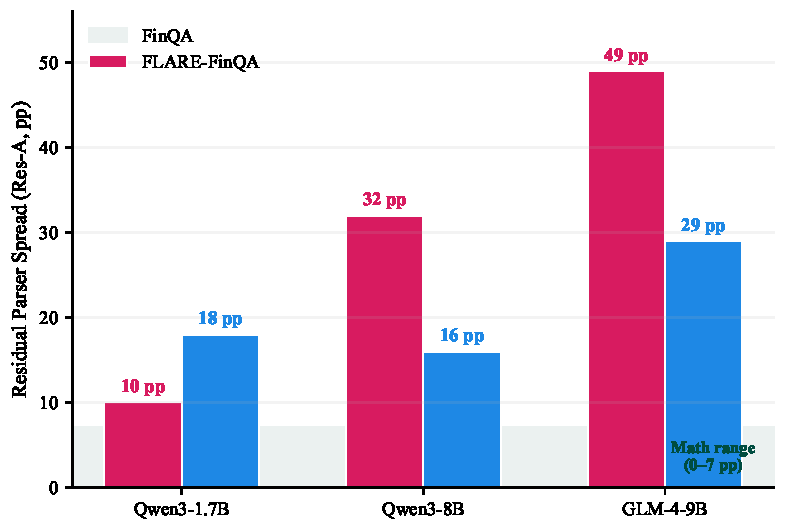
\includegraphics[width=\columnwidth]{figures/figure2_residual_scale.pdf}
\caption{Residual parser spread (Res-A) across models. FinQA spread increases from 10\,pp (Qwen3-1.7B) to 32\,pp (Qwen3-8B); GLM-4-9B (cross-family) reaches 49\,pp. FLARE-FinQA spans 16--29\,pp. The shaded band (0--7\,pp) marks the range observed across all mathematical benchmarks.}
\label{fig:residual_scale}
\end{figure}

Two layers are visible in Table~\ref{tab:cross_domain}. \textbf{Layer~1: the \numparser{} parser fails on every benchmark.} The full spread---max $-$ min across all five parsers---ranges from 16\pp{} (FLARE 8B) to 87\pp{} (GSM8K 8B) across all conditions. The largest gap occurs on a mathematical benchmark, not a financial one. Format mismatch between parser assumption and model output convention is a universal evaluation problem.

\textbf{Layer~2: residual sensitivity differs by domain.} The primary metric is Res-B (excluding both \numparser{} and \boxedparser{}): financial benchmarks show 3--19\pp{}, versus 1--7\pp{} on mathematical controls. Res-A (excluding only \numparser{}) ranges from 10--49\pp{}, but it includes the potentially format-specific \boxedparser{} parser and is inflated by \boxedparser{} incompatibility---GLM scores 0\% on \boxedparser{}, which alone contributes 49\pp{} of that range. On math, once the format is correctly handled, all reasonable parsers agree within single-digit percentages (1--7\pp{} under both Res-A and Res-B). On finance, parser choice continues to move accuracy substantially, though the degree varies by benchmark and residual definition.

\begin{figure}[htb!]
\centering
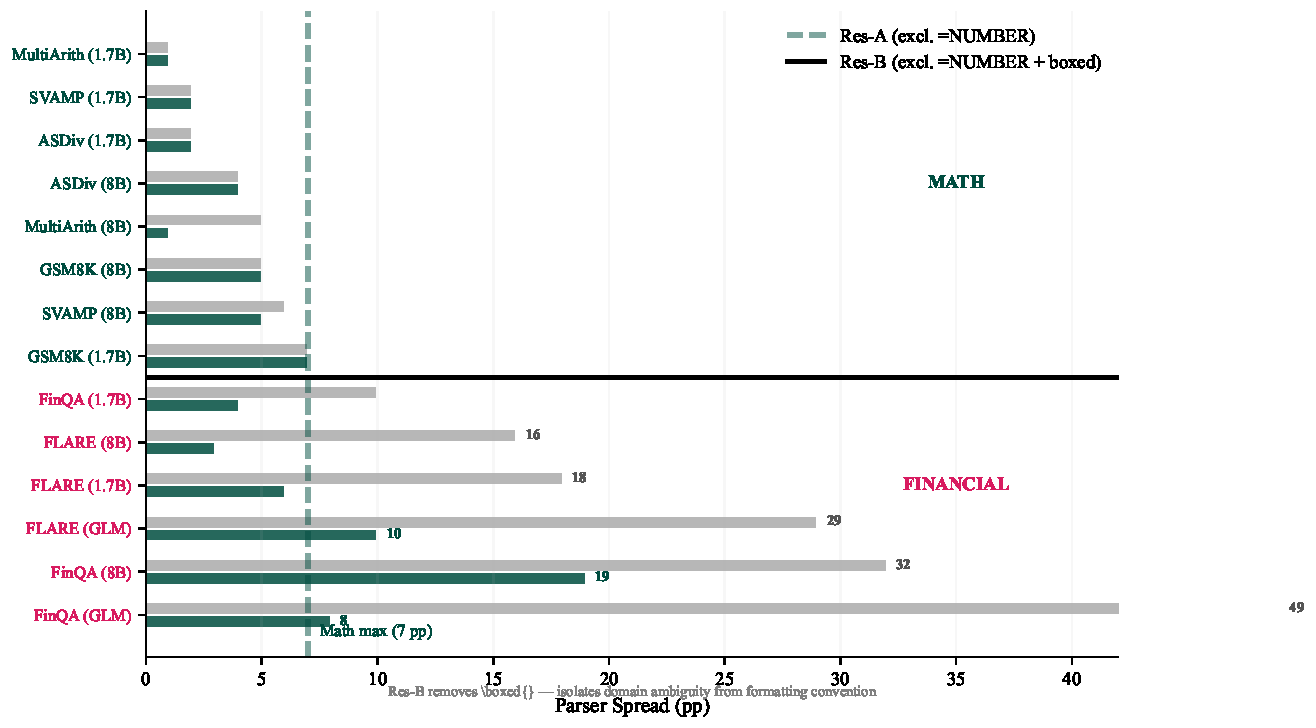
\includegraphics[width=\columnwidth]{figures/figure4_resA_resB.pdf}
\caption{Res-A versus Res-B: isolating domain-level parser sensitivity from format-convention effects. Light gray bars show Res-A (excluding only \numparser{}); dark green bars show Res-B (excluding both \numparser{} and \boxedparser{}). Financial benchmarks retain elevated sensitivity under Res-B on the largest-effect conditions (FinQA 8B at 19\,pp, FLARE GLM at 10\,pp). Some financial conditions narrow to math-like levels under Res-B (FLARE 8B 3\,pp, FinQA GLM 8\,pp).}
\label{fig:resAB}
\end{figure}

Table~\ref{tab:cross_domain} also reports \textbf{Res-B} (excluding both \numparser{} and \boxedparser{}), which isolates domain-level ambiguity from format-convention effects. Under Res-B, financial spreads narrow but remain elevated on the largest-effect conditions (FinQA 8B at 19\,pp, FLARE GLM at 10\,pp). Some financial conditions narrow to math-like levels (FLARE 8B 3\,pp, FinQA GLM 8\,pp), suggesting partial format-driven sensitivity. The core finding holds: on FinQA 8B (19\,pp Res-B), the effect survives removing \boxedparser{}.

\textbf{Scale and cross-family effects.} On FinQA, the residual spread increases from 10\pp{} (Qwen3-1.7B) to 32\pp{} (Qwen3-8B), and reaches 49\pp{} for the cross-family GLM-4-9B model. This pattern---the effect is not specific to a single architecture ---is corroborated on FLARE-FinQA (18\pp{}, 16\pp{}, 29\pp{} for 1.7B, 8B, GLM).

\textbf{Sampling uncertainty.} We bootstrap 95\% confidence intervals for Res-A and Res-B spreads over benchmark items (10K resamples). For Res-A, FinQA 8B yields 32.0\,pp CI~[23.0,\,42.0] versus GSM8K 8B 5.0\,pp CI~[1.0,\,10.0]; the CIs do not overlap. FinQA 1.7B (10.0\,pp, CI~[4.0,\,17.0]) overlaps with GSM8K 1.7B (7.0\,pp, CI~[2.0,\,12.0]). For Res-B, FinQA 8B yields 19.0\,pp CI~[11.0,\,27.0] versus GSM8K 8B 5.0\,pp CI~[1.0,\,10.0]; again the CIs do not overlap. FinQA 1.7B (4.0\,pp, CI~[1.0,\,10.0]) and GSM8K 1.7B (7.0\,pp, [2.0,\,12.0]) overlap substantially with no significant difference.

To directly test whether the Res-B gap between financial and mathematical benchmarks is significant, we compute the bootstrap distribution of the difference between independent two-sample resamples (FinQA $-$ GSM8K, 10K iterations). For the 8B models, the difference is 14.1\,pp, 95\% CI~[5.0,\,23.0]\,pp, which excludes zero ($p = 0.001$). For the 1.7B models, the difference is $-2.5$\,pp, CI~[$-$9.0,\,5.0]\,pp, not significant ($p = 0.77$). The Res-A difference is also significant for 8B (26.9\,pp, CI~[16.0,\,38.0]\,pp) but not for 1.7B. Thus the sensitivity difference between FinQA and GSM8K is statistically robust at the 8B scale for both residual definitions; the 1.7B models, with lower baseline accuracy, do not show a significant domain gap.

\textbf{Oracle upper bound.} We compute the oracle accuracy achievable by multi-parser aggregation: an answer is counted correct if \emph{any} of the five parsers extracts the correct answer. The oracle improves over the best single parser by only 1--2\,pp on FinQA and 0--1.0\,pp on GSM8K. While parser choice materially affects measured accuracy, parser ensembling alone cannot close the main performance gap; 47--58\% of FinQA items are missed by all five parsers simultaneously, confirming that model reasoning capability, not extraction method, is the dominant absolute bottleneck on these benchmarks.

\textbf{No single parser is optimal across financial benchmarks.} On FinQA, \texttt{last\_number} wins by substantial margins in all model conditions. On FLARE-FinQA, \texttt{fixed} wins on 1.7B and GLM, while \texttt{last\_number} wins on 8B. These benchmarks both target financial numerical reasoning, yet their optimal extraction strategies differ. There is no single correct parser for financial evaluation; multi-parser evaluation should become standard practice.

\textbf{Parser choice changes who wins.} We compute rank correlations (Kendall $\tau$) between parser-induced model orderings. On FinQA, the winner changes from Qwen3-1.7B under \numparser{} and \boxedparser{} to GLM-4-9B under the other three parsers---a complete reversal of the top-ranked model. The extreme case is \numparser{} vs.\ \texttt{last\_number}: $\tau = -1.00$ (Spearman $\rho = -1.00$), meaning the model ranking is perfectly inverted (all three model pairs swap order). Even among the three reasonable parsers, \texttt{fixed} vs.\ \texttt{last\_number} has $\tau = +0.33$ ($\rho = +0.50$) with 1 of 3 model pairs reversing order, while \texttt{fixed} and \texttt{finance\_aware} agree perfectly ($\tau = +1.00$). On FLARE-FinQA, rankings are more stable: Qwen3-1.7B is top-ranked or tied under all five parsers, and pairwise $\tau$ ranges from +0.33 to +1.00 with at most 1 reversal per pair. This asymmetry---FinQA rankings are parser-sensitive, FLARE rankings are more robust---is itself evidence that benchmark design choices affect extraction sensitivity.

\textbf{Cross-family validation.} To confirm that extraction sensitivity is not specific to the Qwen3 architecture, we evaluated GLM-4-9B-Chat~\cite{glm2024} on both financial benchmarks. GLM reproduces the qualitative pattern: its Res-A spread reaches 49\,pp on FinQA, the largest value observed. Under Res-B (excluding \boxedparser{}, which scores 0\% because GLM never uses \LaTeX{} formatting), the spreads are 8\,pp and 10\,pp---still comparable to or larger than the math range. This confirms that \boxedparser{} extraction depends on model-specific output conventions, and that cross-family validation must account for format compatibility.

\subsection{Matched Counterfactual: Stripping Financial Surface Forms}
\label{sec:counterfactual}

To isolate the role of financial surface forms from output-format conventions, we run a counterfactual ablation: we take the model outputs for FinQA 8B and FLARE 8B, strip all financial formatting (currencies, percentages, magnitudes, accounting negatives) from the response text, and re-apply the same five parsers. If financial formats are what make the parsers disagree, stripping them should narrow the Res-B gap; if a domain-aware parser was using those formats correctly, stripping them can instead increase disagreement by removing that advantage.

On FinQA 8B, the Res-B gap narrows from 19.0\,pp to 11.0\,pp after stripping, with 14 of 500 extraction decisions changing. Financial surface forms account for approximately 8\,pp of the 19\,pp gap, while the remaining 11\,pp persists after stripping. Combined with the supplementary audit of Res-B disagreements (Section~\ref{sec:finance_challenges}), the residual 11\,pp is driven by output-level conventions---multi-step extraction position, gold-answer normalization, and sign formatting---rather than the \boxedparser{}-style format mismatch that inflates Res-A.

On FLARE 8B, the opposite occurs: Res-B \emph{increases} from 3.0\,pp to 10.0\,pp after stripping. The mechanism is that \texttt{finance\_aware} correctly interprets financial surface forms in the original outputs, and stripping them removes its advantage, causing it to disagree more with the other parsers. This asymmetry---FinQA sensitivity is driven by output-level conventions, while FLARE exposes the benefit of finance-aware normalization---explains why the two benchmarks show different residual spread profiles and confirms that domain-aware parsing matters when outputs contain financial formats.

\subsection{Finance-Specific Failure Taxonomy}

We conducted a manual audit of 104 model responses on FinQA, classifying extraction failures into six categories: format mismatch (40\%), magnitude confusion (15\%), multi-step extraction (15\%), currency prefix stripping (12\%), percentage normalization (10\%), and sign convention errors (8\%). Full details including annotation protocol, inter-annotator agreement, and per-category examples are in Section~\ref{sec:finance_challenges}. The four finance-specific categories (magnitude, currency, percentage, sign) account for 45\% of failures. Combined with the cross-domain comparison, these categories explain why financial benchmarks retain elevated residual sensitivity even after format mismatch is controlled: parsers must handle domain-specific numeric conventions that do not appear in standard math problems.

\section{Discussion}
\label{sec:implications}

The results in Section~\ref{sec:results} show that answer extraction is not a solved problem but an active source of measurement error in financial LLM evaluation. We outline implications for benchmark designers and practitioners, and propose a concrete reporting protocol.

\subsection{For Benchmark Designers}
\label{sec:impl_benchmark}

An accuracy number reported without specifying the extraction method is incomplete. Our experiments show that the choice of parser can shift accuracy by up to 87\pp{} (Table~\ref{tab:cross_domain}) and that the optimal parser differs across financial benchmarks even within the same domain. The ecosystem audit (Section~\ref{sec:parser_audit}) further reveals that no shared extraction standard exists and that several frameworks do not fully document their procedures. For benchmark designers, this means that extraction methodology must be treated as part of the measurement instrument: it should be specified, released, and tested for sensitivity, just as the evaluation dataset and metric are. We provide a concrete protocol in Section~\ref{sec:protocol}.

\subsection{Operational and Governance Implications}
\label{sec:impl_operations}

Parser sensitivity has practical consequences for model selection and deployment. Our FinQA results show that model rankings depend on parser choice: a practitioner selecting a model from a published leaderboard has no guarantee that the benchmark's extraction method matches their production pipeline. If rankings change between parsers, the benchmark is measuring the interaction between output format and parser logic rather than financial reasoning ability, and deployment decisions should be based on task-specific evaluation with the production parser.

A concrete example illustrates the magnitude of the risk. A model validated at 44\% accuracy on FinQA (Qwen3-8B under \texttt{last\_number}) could operate at 11\% accuracy if the production pipeline uses a different parser (the \numparser{} result on the same outputs)---a 33\,pp drop with no change to the model itself. This gap is relevant to model governance: the EU AI Act~\cite{euaiact} requires accuracy testing suitable for the intended purpose, and emerging financial regulatory guidance emphasizes that validation should reflect conditions of use~\cite{sr2602}. While we do not make legal conclusions, the example illustrates how extraction pipelines, which are rarely version-controlled, can introduce undisclosed divergence between tested and deployed system behavior.

\subsection{Recommended Extraction Protocol}
\label{sec:protocol}

Based on our findings, we recommend the following protocol for financial LLM evaluation:

\begin{enumerate}
    \item \textbf{Canonical answer format.} Benchmarks should prescribe a specific answer format (e.g., final numeric value on the last line, or a structured schema) that models are expected to produce. This makes the extraction contract explicit and uniform across models---unlike per-model native-format selection, which would introduce model-dependent measurement instruments and reduce leaderboard comparability.
    \item \textbf{Structured output as primary metric.} Where feasible, use constrained decoding or structured output APIs to enforce the canonical format. When constrained decoding is unavailable, report the format compliance rate alongside accuracy.
    \item \textbf{Multi-parser sensitivity as a diagnostic.} Report accuracy under at least two extraction methods (e.g., the canonical parser and a format-agnostic fallback). The spread between them is a diagnostic of extraction robustness, not a second accuracy number.
    \item \textbf{Disagreement auditing.} Flag questions where the canonical and fallback parsers disagree for manual review. A high disagreement rate signals that extraction noise affects the reported error rate.
\end{enumerate}

We emphasize that multi-parser sensitivity reporting is a diagnostic tool, not a replacement for a well-defined evaluation contract. Our oracle analysis shows that even perfect multi-parser aggregation improves accuracy by only 1--2\,pp, so investment should go toward canonical formats rather than increasingly sophisticated post-hoc parsers.

\section{Conclusion}
\label{sec:conclusion}

Answer extraction is an uncontrolled measurement variable in financial LLM evaluation, not a trivial implementation detail. Across two financial benchmarks and three models, parser choice shifts reported accuracy by up to 19\,pp among format-compatible methods, compared with 1--7\,pp on mathematical controls. The root cause is benchmark-dependent, involving both financial surface forms and output-level conventions such as multi-step reasoning traces and answer normalization. No single parser is optimal, and rankings can invert across parsers. The primary practical implication is that benchmarks should adopt canonical answer formats as their primary evaluation contract, with multi-parser sensitivity reported as a diagnostic rather than a substitute.


\bibliographystyle{ACM-Reference-Format}
\bibliography{references}

\end{document}
